\section{Status of Experiments}

I am trying to use the same neural network architecture as Schaurecker et al.\cite{schaurecker_super-resolving_2021}. Schaurecker et al. have open sourced their code. \footnote{Source is available at \url{https://github.com/dschaurecker/dl_halo/}}

\begin{figure}[h!]
  \begin{centering}
    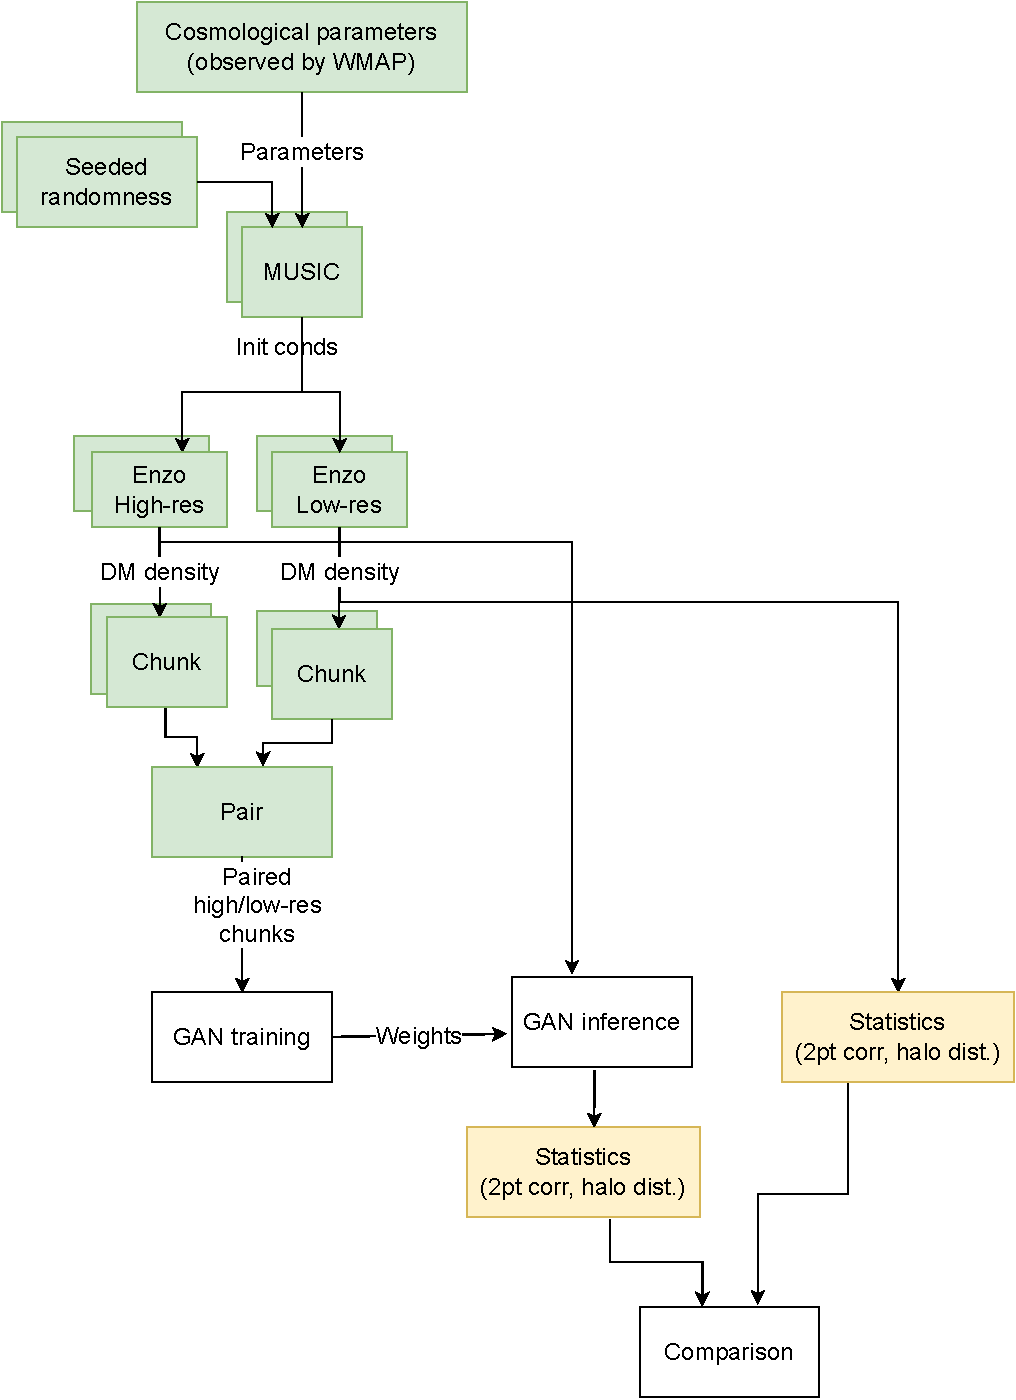
\includegraphics[width=0.7\textwidth]{./astrophysics-experiment-status.pdf}
  \end{centering}
  \caption{This figure shows the computational tasks in the experiment.}
  \label{workflow}
\end{figure}

Recall my experimental setup summarized in \cref{workflow}. I have written a script that can preform the green tasks in an automated fashion. I have partially implemented the yellow tasks. I have yet to implement the white tasks.

\section{Problems}

More work needs to be done to put the output of Enzo into a format that can be processed by the map2map\footnote{Source is available at \url{https://github.com/eelregit/map2map}} neural network library. Map2map requires that the AMR data be sampled desnely and split into equal-sized rectangular chunks with padding. 

I have been unable to install PyTorch on the campus cluster with CUDA. I have tried using the conda package manager, but it seems there is a diamond dependency conflict between the CUDA version of PyTorch and yt, another package I need to do this analysis.

Additionally, the FoaF halo finder requires the generated density field be resampled into individual particles. This is the opposite of CIC interpolation.

% TODO: Elaborate

\section{Simulation Output}

\begin{figure}[h!]
  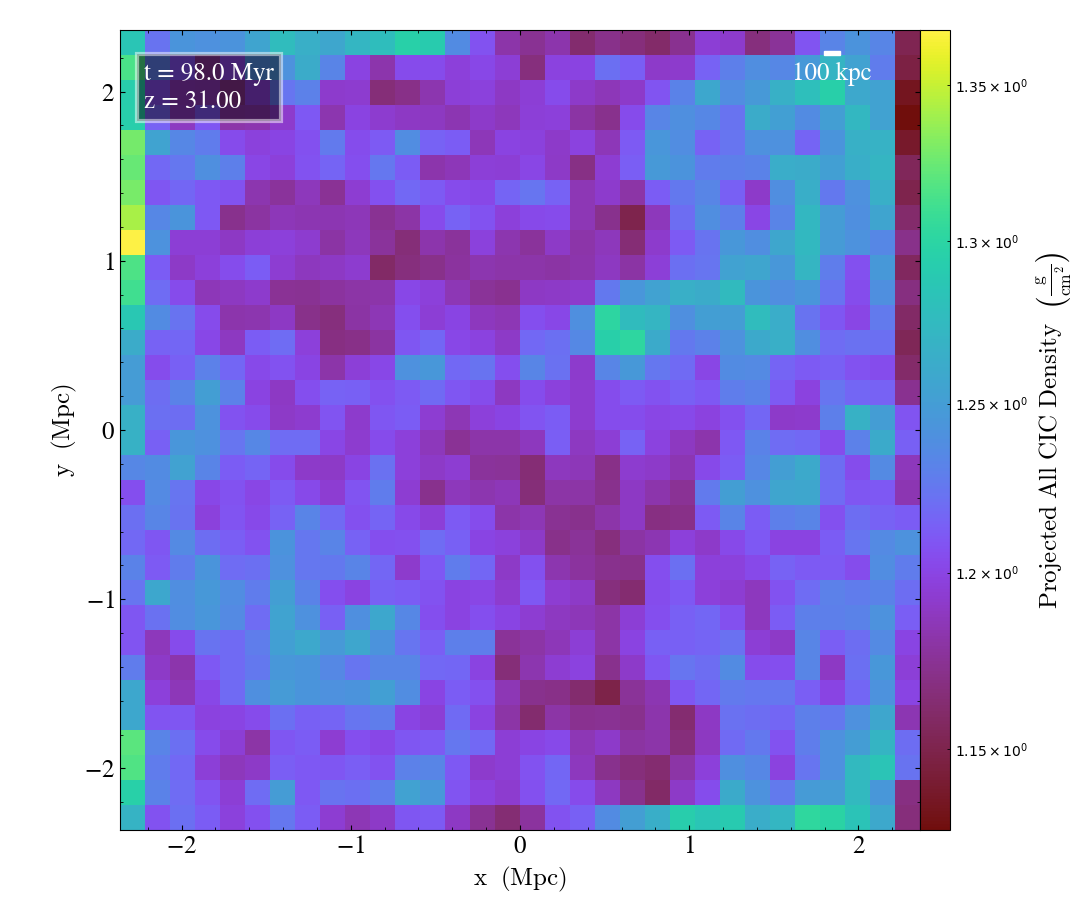
\includegraphics[width=0.45\textwidth]{../../presentation/assets/sim-0.png}
  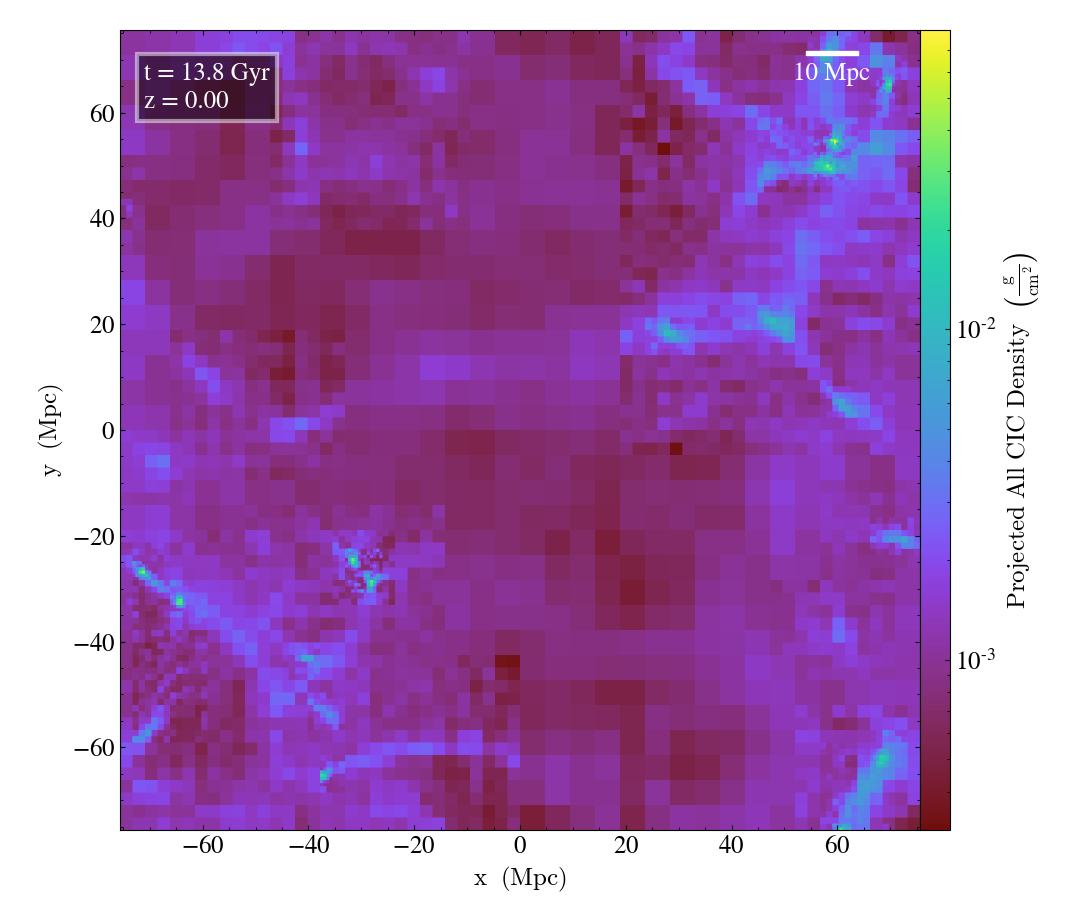
\includegraphics[width=0.45\textwidth]{../../presentation/assets/sim-1.png}
  \label{cosmology-result}
  \caption{This plot shows the dark matter density integrated along the Z-axis at the beginning of the simulation (left) and at the end (right) in comoving coordinates.}
\end{figure}

I believe that generating initial conditions with MUSIC \cite{hahn_multi-scale_2011} and simulating them with Enzo \cite{collins_cosmological_2010,bryan_enzo_2014} is working correctly based on the images in \cref{cosmology-result}. They show dark matter initially smeared out evenly across the universe (left figure) at z = 31, 98 Myr after the big bang. Then dark matter condenses into filaments and halos at z = 0, present day. One can see the adaptive mesh refine in ``interesting'' areas. Also note that the simulation region has physically expanded due to Hubble expansion.

% TODO: Low vs high res

\section{Limitations of this approach}

Most well studied neural net operates on a field sampled at a regular grid, not an AMR grid. As such, the AMR output of Enzo has to be interpolated into a fixed grid. This ends up losing the advantages that the AMR had in the first place. If one uses the finest granularity everywhere, the sampling uses an extravagant amount of memory; if one uses a coarser resolution, the sampling fails to capture all of the details. This is particularly bad for cosmological simulations where there are extremely intricate halos and filaments surrounded by massive voids. It would be ideal if this neural networks could work natively on AMR grids, but this is a less well-studied case. With regular grids, we can reuse established building-blocks like the U-net and the concept of convolutional layers.

The prior literature \cite{schaurecker_super-resolving_2021,li_ai-assisted_2021} do not define explicit criteria for accepting or rejecting their superresolution approximation. They compare the power spectra, halo mass function, and halo two-point correlation functions graphically. It is difficult to know if an approximation is going to be acceptable without knowing what downstream analysis it is used in.

\section{Simulation Applicability}

This approach to simulating cosmology relies on standard assumptions in \(\Lambda\)CDM. Following Schaurecker et al. \cite{schaurecker_super-resolving_2021}, this simulation neglects baryonic contributions to gravity formation. According to the Wilkinson Anisotropy Probe, baryonic matter only accounts for 4 -- 5\% of the mass-energy in the universe, while dark matter and dark energy accounts for the rest \cite{hinshaw_nine-year_2013}. Enzo assumes Newtonian gravity because the relativistic correction is small so long as the simulation size (100 Mpc ~ \(3 \times 10^{15}\) meters) is small compared to \(c / H = 1.4 \times 10^{26}\) meters) \cite{bryan_enzo_2014}.

\section{Reproducibility}

I have attempted to make my code as reproducible as possible.

\section{Lessons Learned}
